\chapter{Хэрэгжилт ба үр дүн}
\label{Chapter5}

\section{Хэрэгжилтийн ерөнхий үр дүн}

Төслийн бодит хэрэгжилтээр Facebook өгөгдөл цуглуулах, хадгалах, API-аар түгээх, dashboard дээр хянах, Gemini-ээр тайлан үүсгэх үндсэн workflow бүрэн бүрдсэн.

\begin{table}[H]
\centering
\caption{Хэрэгжсэн модулиудын нэгтгэл}
\small
\renewcommand{\arraystretch}{1.25}
\begin{adjustbox}{max width=\textwidth}
\begin{tabular}{|p{3.6cm}|p{9.8cm}|}
\hline
\rowcolor{gray!20}\textbf{Модуль} & \textbf{Бодит үр дүн} \\
\hline
Frontend dashboard & Live backend posts/statistics унших, demo fallback харуулах, chart болон recent post cards гаргах \\
\hline
Data source manager & \texttt{pages.txt} target list унших/хадгалах, scraper run/status/log endpoint ашиглах \\
\hline
Admin control & Backend health, stats, posts snapshot харуулах, browser-side keyword/date/platform filter хийх \\
\hline
FastAPI backend & Posts, comments, images, stats, sentiment, topics, trends, sheets export, Gemini, scraper control endpoint-ууд \\
\hline
Scraper & Facebook target list унших, Selenium/BeautifulSoup workflow ажиллуулах, log file үүсгэх \\
\hline
Database & PostgreSQL/SQLAlchemy model, duplicate-aware save, analysis result storage \\
\hline
Analysis & TextBlob/basic sentiment, LDA topic modeling, engagement score/prediction \\
\hline
AI report & Gemini API ашиглан recent data summary-аас Монгол хэл дээр тайлан, зөвлөмж үүсгэх \\
\hline
\end{tabular}
\end{adjustbox}
\normalsize
\end{table}

\section{Хэрэглэгчийн интерфэйс болон функцүүдийн хэрэгжилт}

Frontend нь хэрэглэгчид шууд харагдах үндсэн ажлын талбар болсон. Dashboard нь backend өгөгдөлтэй холбогдсон үед "Live mode", холбогдохгүй үед "Demo mode" гэж ялган харуулдаг. Энэ нь demo presentation болон backend availability хоёр нөхцөлийг нэг UI-аар даах боломж өгсөн.

\subsection{Data Sources болон Scraper Control}
Хэрэглэгч Data Sources цонхонд нэвтэрч Facebook хуудасны URL оруулан scraping процессыг удирдана. Automation console нь scraper-ийн log-ийг шууд дэлгэцэнд харуулдаг.

\begin{figure}[H]
\centering
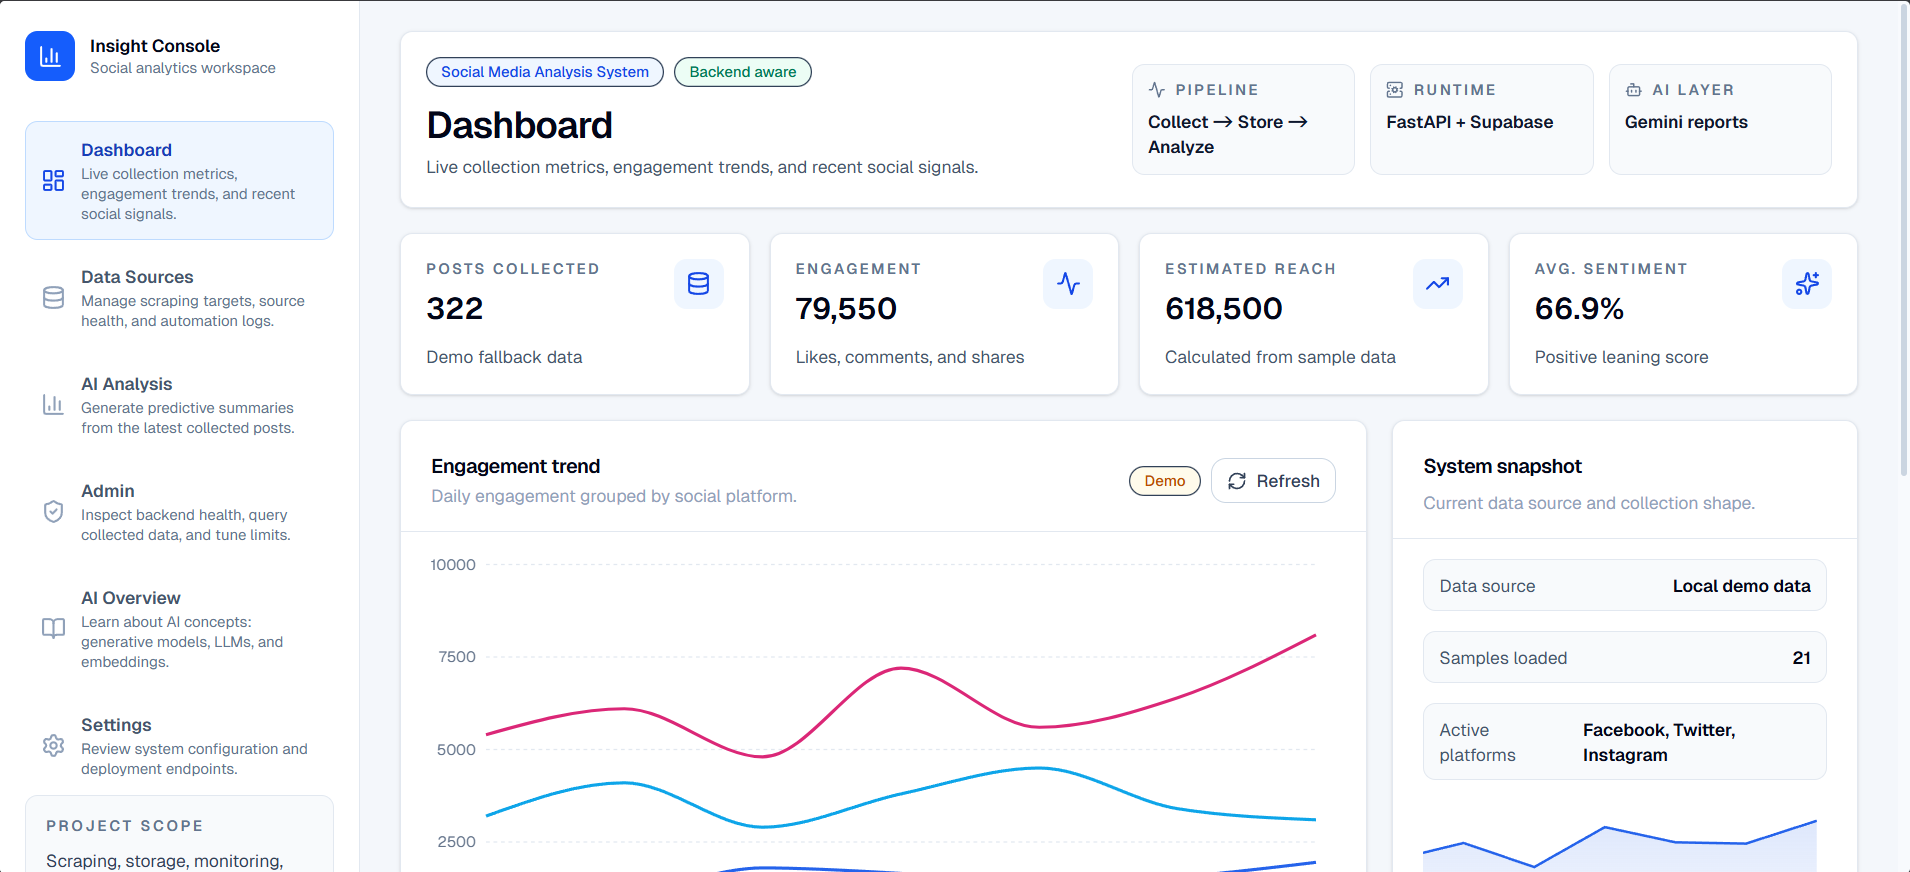
\includegraphics[width=0.9\textwidth]{Figures/dashboard1.png}
\caption{Data Sources цонх болон Automation Console}
\label{fig:data_sources_ui}
\end{figure}

\subsection{Үндсэн Dashboard болон Үзүүлэлтүүд}
Dashboard хэсэгт нийт цуглуулсан постын тоо, engagement score, sentiment analysis-ийн дундаж үзүүлэлт зэргийг товчоор харуулна. Мөн хугацаанаас хамаарсан оролцооны графикийг (Engagement trend) Recharts ашиглан зурж харуулдаг.

\begin{figure}[H]
\centering
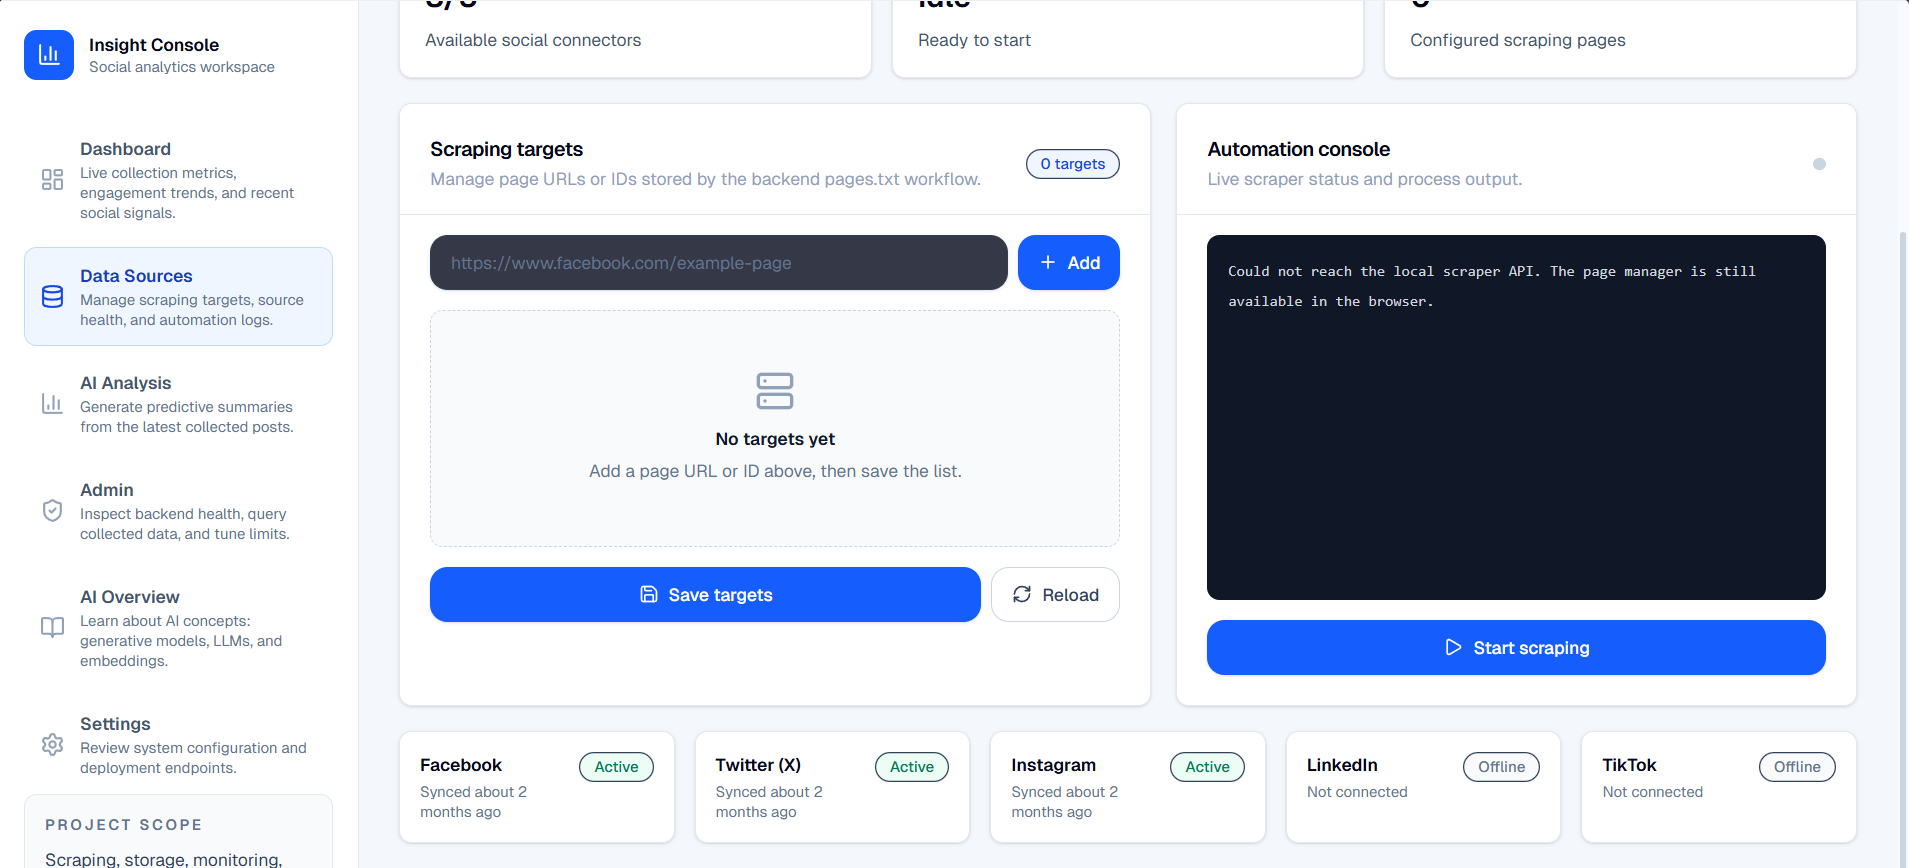
\includegraphics[width=0.9\textwidth]{Figures/dashboard2.png}
\caption{Үндсэн Dashboard болон Engagement trend}
\label{fig:main_dashboard}
\end{figure}

\subsection{Admin Control болон Хяналт}
Admin panel нь системийн тохиргоо болон хязгаарлалтыг удирдах хэсэг юм. Эндээс backend server-ийн төлөв (status), өгөгдлийн сангийн холболт болон хэдэн пост, сэтгэгдэл татах limit зэргийг тохируулж болно.

\begin{figure}[H]
\centering
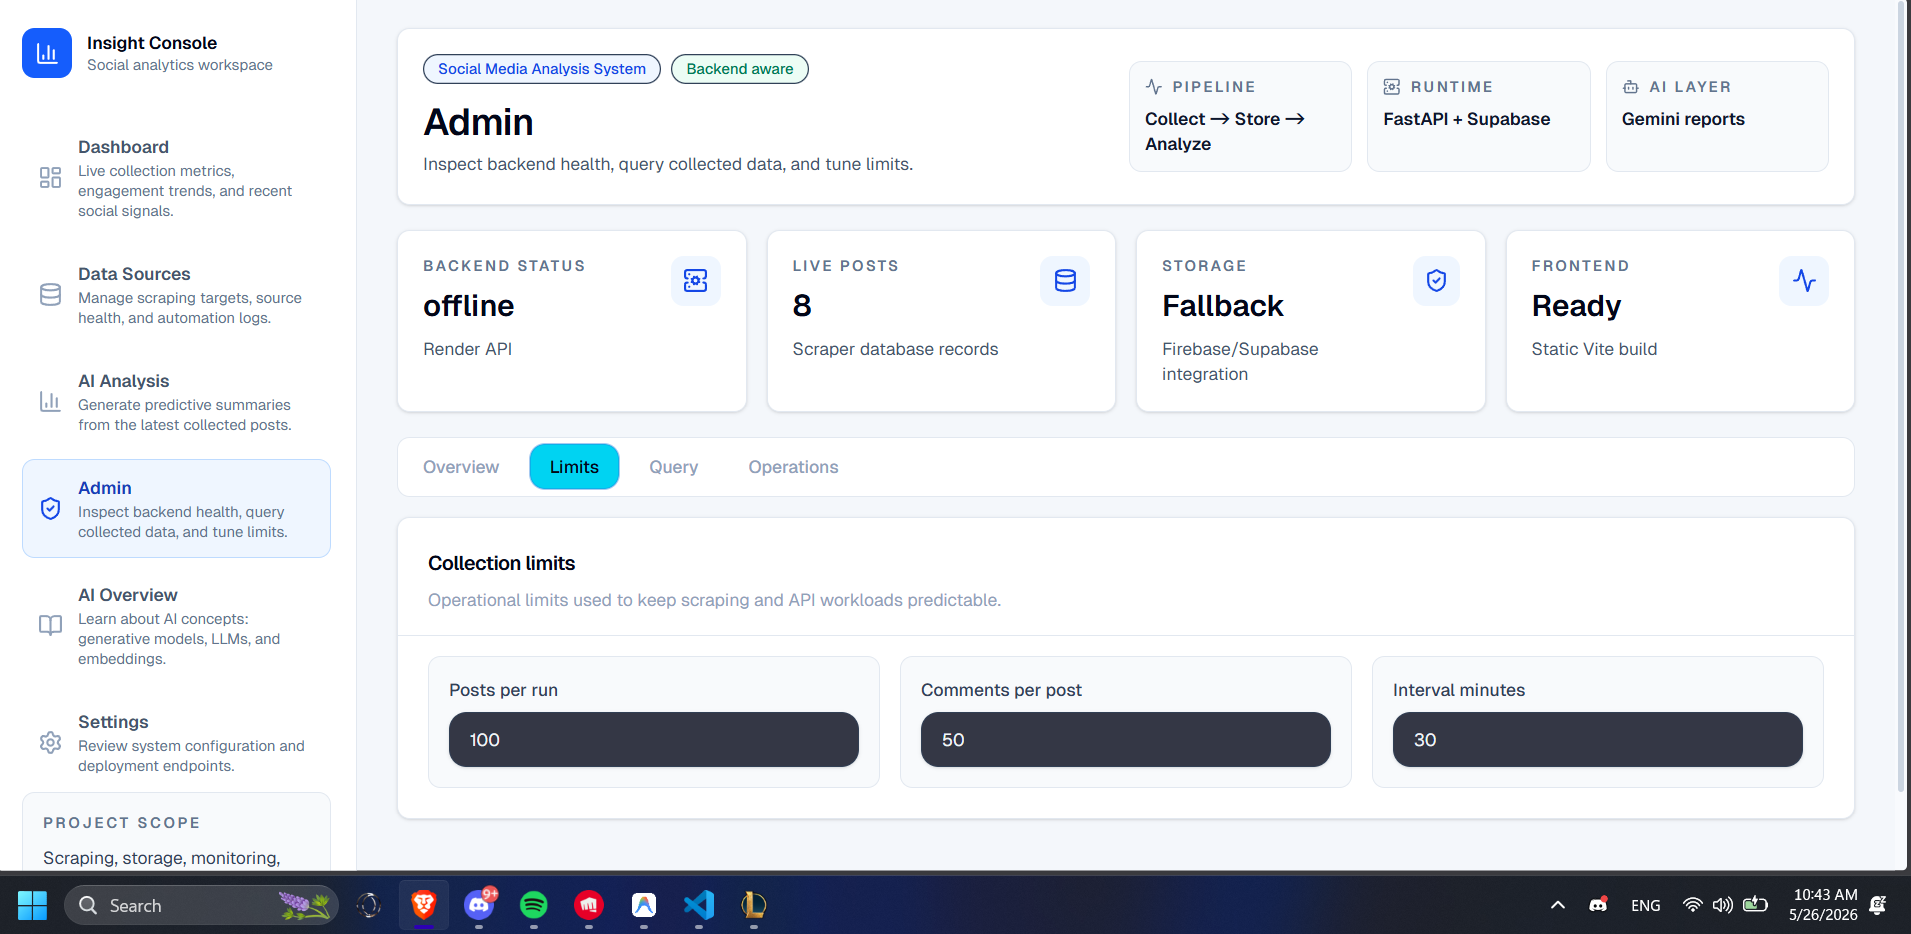
\includegraphics[width=0.9\textwidth]{Figures/admin1.png}
\caption{Admin Control болон Backend Status}
\label{fig:admin_control}
\end{figure}

\begin{figure}[H]
\centering
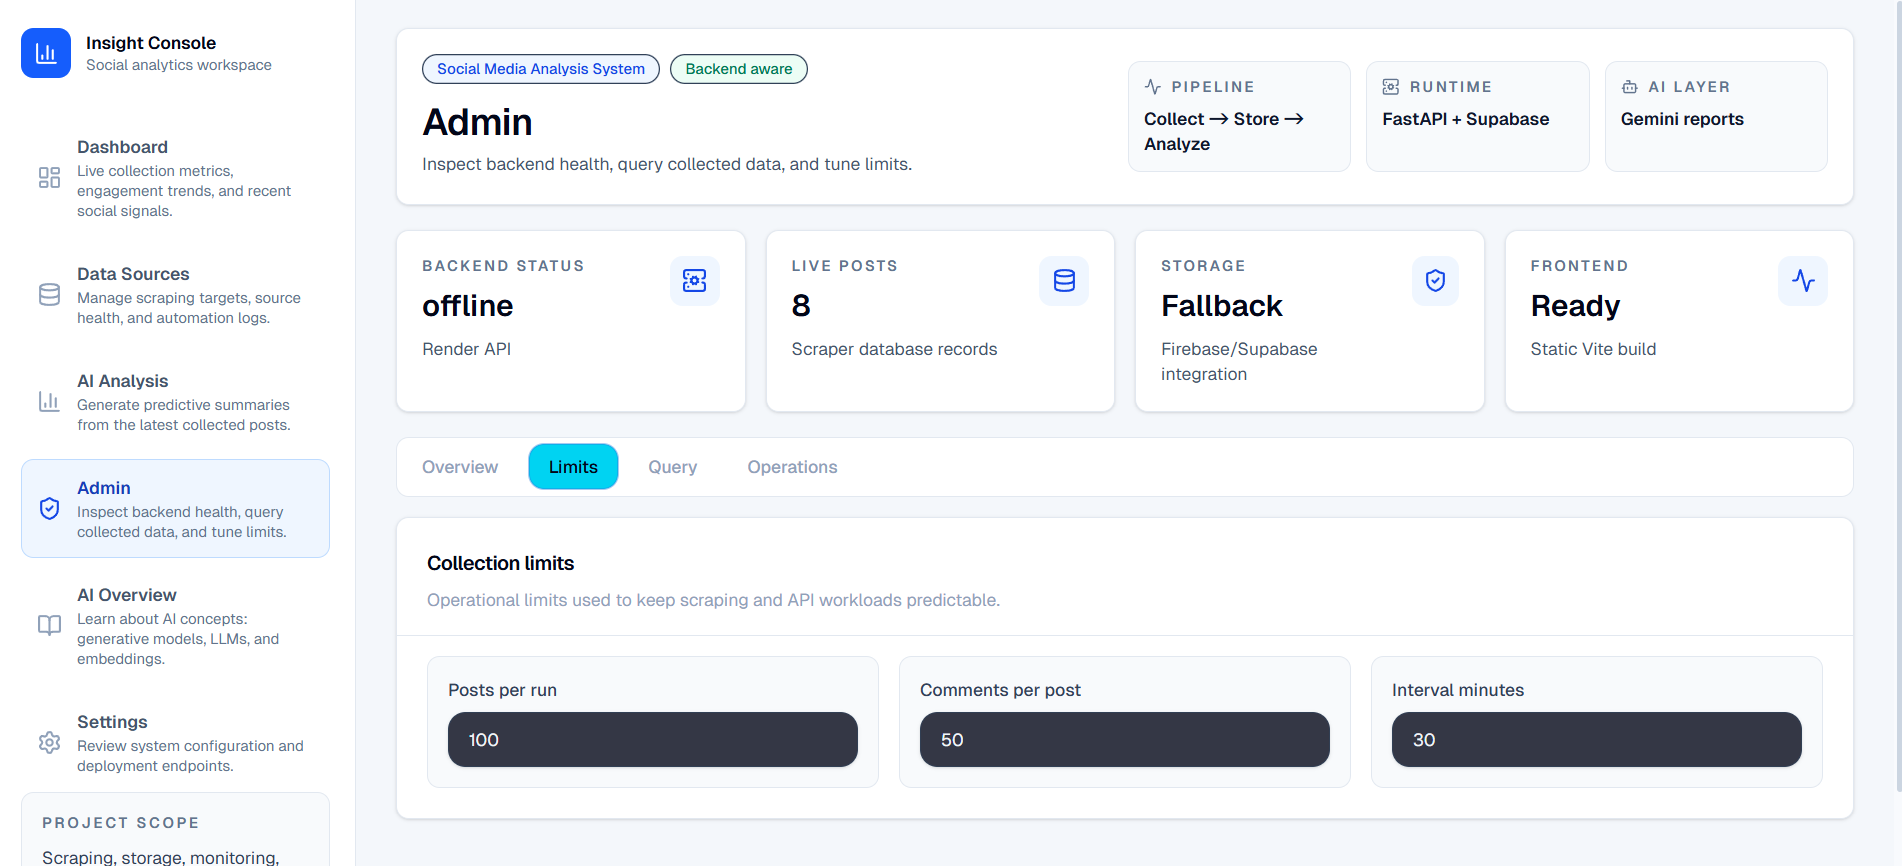
\includegraphics[width=0.9\textwidth]{Figures/admin2.png}
\caption{Collection limits (Хязгаарлалтын тохиргоо)}
\label{fig:admin_limits}
\end{figure}

\section{Туршилтын үр дүн ба баталгаажуулалт}

Системийн функциональ шаардлагууд хэрхэн хангагдсаныг доорх байдлаар шалгаж баталгаажуулав.

\begin{table}[H]
\centering
\caption{API workflow баталгаажуулалт}
\small
\renewcommand{\arraystretch}{1.25}
\begin{adjustbox}{max width=\textwidth}
\begin{tabular}{|p{3.6cm}|p{9.8cm}|}
\hline
\rowcolor{gray!20}\textbf{Workflow} & \textbf{Үр дүн} \\
\hline
Health check & Database/analyzer/sheets/gemini initialization flag амжилттай буцаана. \\
\hline
Posts/statistics & Dashboard-д хэрэгтэй post list, total posts, total pages, total comments, average metrics зөв буцаж байна. \\
\hline
Scraper control & Target list унших/бичих, scraper process эхлүүлэх, active status, log tail буцаах үйлдлүүд хэвийн ажиллаж байна. \\
\hline
Analysis & Sentiment, topic, engagement result-уудыг post бүр дээр тооцоолж мэдээллийн санд хадгалсан. \\
\hline
Gemini & Backend environment-д API key тохируулсан үед summary/Q\&A prompt амжилттай ажиллаж тайлан гаргаж байна. \\
\hline
\end{tabular}
\end{adjustbox}
\normalsize
\end{table}

\section{Үр дүнгийн хэлэлцүүлэг}

Судалгааны эхэнд тавьсан асуултуудын хүрээнд:
\textbf{RQ1-ийн хүрээнд:} Selenium болон BeautifulSoup ашигласан scraper workflow, target list, log management хэрэгжсэн тул Facebook өгөгдөл цуглуулах үндсэн pipeline амжилттай бүрдсэн.
\textbf{RQ2-ийн хүрээнд:} FastAPI endpoint-ууд болон React dashboard нь live backend data-г chart, card, query view хэлбэрээр хэрэглэгчид хүргэж байна. Backend unavailable үед demo fallback ажилладаг нь presentation болон хөгжүүлэлтийн үед маш хэрэгтэй болсон.
\textbf{RQ3-ийн хүрээнд:} TextBlob/basic sentiment, LDA topic modeling, engagement score, Gemini report generation нь өгөгдлийг зөвлөмж болгон хувиргах эхний шатны pipeline үүсгэсэн. Ингэснээр цуглуулсан хуурай өгөгдлийг тайлан болгож хувиргах автоматжуулалт бий боллоо.

\section{Хязгаарлалт ба эрсдэл}
\begin{itemize}
    \item Facebook UI өөрчлөгдөхөд selector болон modal handling эвдрэх эрсдэлтэй.
    \item Backend болон frontend-д зарим текст encoding алдаа (Монгол фонт) гарч болзошгүй.
    \item Gemini report нь API key болон network availability-аас хамаарна.
    \item Бусад платформын (Instagram, TikTok) scraper болон deep-learning sentiment model нь энэ хувилбарт бүрэн хэрэгжээгүй.
\end{itemize}
